\section{Evaluation with Java Projects}
\label{sec:eval:java}

\begin{figure*}[htpb]
\centering
%\includegraphics[width=0.8\textwidth]{img-diff3.pdf}
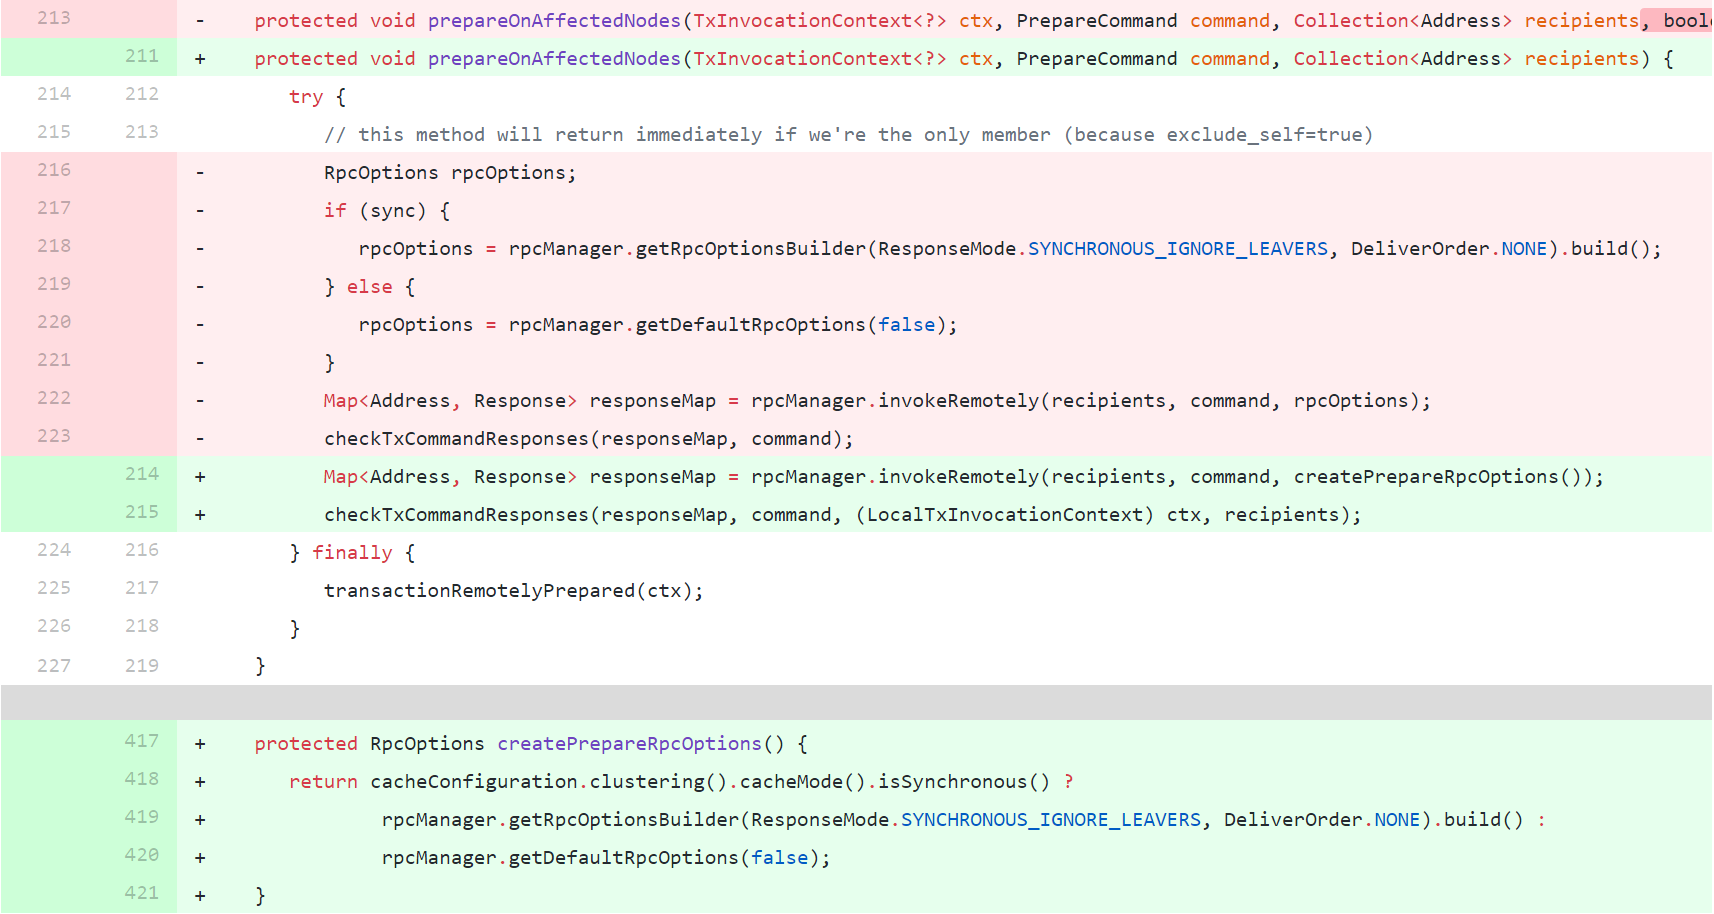
\includegraphics[width=1.0\textwidth]{img-ex-new-extract-infinispan-ce4f629.png}
\caption{Illustrative diff of an \emph{Extract Method} refactoring considered as true positive by the validators, taken from commit ce4f629 from \emph{infinispan} project.}
\label{FigDiff3}
\end{figure*}


\begin{table*}[htbp]
\renewcommand{\arraystretch}{1.2}
\caption{Java precision and recall results}
\label{TabResultJava}
\centering
\begin{tabular}{@{}lrlrrrlllrrrll@{}}
\toprule
 & & & \multicolumn{2}{c}{RefDiff 1.0} & & \multicolumn{2}{c}{RefDiff 2.0} & & \multicolumn{2}{c}{RMiner 1.0}\\
\cmidrule{4-5} \cmidrule{7-8} \cmidrule{10-11}
Refactoring Type & \# & & Precision & Recall & & Precision & Recall & & Precision & Recall \\
\midrule
Move Class & 1100 & & \xbar{0.999} & \xbar{0.881} & & \xbar{0.999} & \xbar{0.970} & & \xbar{1.000} & \xbar{0.925} \\
Move Method & 319 & & \xbar{0.322} & \xbar{0.746} & & \xbar{0.871} & \xbar{0.803} & & \xbar{0.955} & \xbar{0.658} \\
Move and Rename/Rename Class & 95 & & \xbar{0.897} & \xbar{0.642} & & \xbar{0.922} & \xbar{0.874} & & \xbar{0.983} & \xbar{0.621} \\
Rename Method & 350 & & \xbar{0.855} & \xbar{0.811} & & \xbar{0.946} & \xbar{0.694} & & \xbar{0.978} & \xbar{0.771} \\
Extract Interface & 24 & & \xbar{0.769} & \xbar{0.417} & & \xbar{0.875} & \xbar{0.875} & & \xbar{1.000} & \xbar{0.833} \\
Extract Superclass & 70 & & \xbar{1.000} & \xbar{0.157} & & \xbar{1.000} & \xbar{0.743} & & \xbar{0.958} & \xbar{0.971} \\
Pull Up Method & 91 & & \xbar{0.806} & \xbar{0.593} & & \xbar{0.974} & \xbar{0.824} & & \xbar{1.000} & \xbar{0.791} \\
Push Down Method & 40 & & \xbar{0.950} & \xbar{0.475} & & \xbar{0.950} & \xbar{0.950} & & \xbar{1.000} & \xbar{0.825} \\
Extract/Extract and Move Method & 1037 & & \xbar{0.904} & \xbar{0.833} & & \xbar{0.962} & \xbar{0.663} & & \xbar{0.985} & \xbar{0.768} \\
Inline Method & 122 & & \xbar{0.842} & \xbar{0.787} & & \xbar{0.957} & \xbar{0.721} & & \xbar{0.990} & \xbar{0.795} \\
\addlinespace
Total & 3248 & & \xbar{0.792} & \xbar{0.802} & & \xbar{0.964} & \xbar{0.804} & & \xbar{0.988} & \xbar{0.813} \\
\bottomrule
\end{tabular}
\end{table*}


In this section, we evaluate the precision and recall of our approach using a recently proposed dataset of refactorings performed in real-world Java open-source projects. We also compare its precision and recall with RMiner---the current state-of-the-art tool for detecting refactorings in Java---and RefDiff~1.0, the previous version of our tool.
First, we present our evaluation design (Section~\ref{sec:eval:java:design}) and then we present the results (Section~\ref{sec:eval:java:results}).

\subsection{Evaluation Design}
\label{sec:eval:java:design}

To evaluate the precision and recall of RefDiff~2.0 in Java we initially use an oracle proposed by Tsantalis et al.~\cite{tsantalis2018rminer}.
This oracle includes 3,188 manually-validated refactoring instances, detected in 538 commits from 185 open-source projects, and covering 15 refactoring types.
It is important to emphasize that most commits contain non-refactoring changes interleaved with refactorings, which is the most challenging scenario for refactoring detection tools.
In our evaluation, we also compare RefDiff's precision and recall against RMiner (version~1.0).
For the purpose of the comparison, we restricted the oracle to 11 refactoring types supported by both tools.
Specifically, we excluded \emph{Change Package}, \emph{Move Field}, \emph{Push Down Field} and \emph{Pull Up Field} from the analysis as they are not supported by RefDiff.
Moreover, \emph{Convert Type} and \emph{Change Signature}, although supported by RefDiff, are not evaluated because they are not covered by the oracle.
In total, our modified oracle contains 3,031 confirmed refactoring instances.
Additionally, it also contains 704 refactoring instances classified as false positives in the process of manual validation performed by Tsantalis et al.~\cite{tsantalis2018rminer}.
These instances are used to detect false positives reported by RefDiff, as described in the next paragraph.
%Last, it is worth noting that the \emph{Rename Class} category also includes instances of \emph{Move and Rename Class}. Similarly, the \emph{Extract Method} category also includes instances of \emph{Extract and Move Method}. This measure was necessary because the oracle did not distinguish between those refactorings reliably.

First, we run RefDiff on each commit of the oracle. For each detected refactoring $r$ we checked whether $r$ is in the oracle, which may yield three outcomes: (i) if $r$ is a confirmed refactoring from the oracle, then it is a true positive; (ii) if $r$ is a false refactoring from the oracle, then it is a false positive; (iii) otherwise, $r$ was inspected by two authors of this paper to assess whether it is a false positive or a true positive not covered by the oracle.
This extra manual validation is needed because the initial oracle must not be granted as complete, i.e., including all refactorings performed in the set of analysed commits.
Specifically, it was constructed using a triangulation approach, based on an initial list of refactorings produced by RMiner~1.0 and RefDiff~1.0. For this reason, it might miss true refactorings only detected by RefDiff~2.0. %the improved implementation of RefDiff, described in this paper.

%\begin{figure*}[!t]
%\centering
%\includegraphics[width=0.8\textwidth]{img-diff2.pdf}
%\caption{Illustrative diff of an \emph{Inline Method} refactoring considered as true positive by the validators.}
%\label{FigDiff2}
%\end{figure*}





After following this procedure, RefDiff 2.0 detected 263 new refactoring instances (i.e., not listed in the initial oracle), which were validated by two paper's authors, called here validators. In the case of 175 refactorings (66\%), the validators agreed on their classification, including 138 refactorings labelled as true positives by both validators and 37 labelled as false positives. After this initial and independent validation, the validators discussed together the remaining 88 cases (34\%), to reach an agreement. As a result, 79 refactorings were considered true positives and 9 refactorings were classified as false positives.
%Figure~\ref{FigDiff2} shows a first example of true positive. RefDiff identified an \emph{Inline Method} refactoring, consisting on the substitution of the method named \codeinl{acquireNodeRelationshipCursor}, which was removed in the same commit, by invocations to methods \codeinl{get()} and \codeinl{init()}. We emphasize in this figure the changes that correspond to this refactoring. This indication of refactoring was not listed in the oracle. The validators individually analyzed this commit and both agreed that an \emph{Inline Method} was applied in this commit.
Figure~\ref{FigDiff3} shows an example of a refactoring identified by RefDiff that both validators classified as true positive.
In this case, a developer extracted method \codeinl{createPrepareRpcOptions} from method \codeinl{prepareOnAffectedNodes}.
%Figure~\ref{FigDiff3} shows an example of a true positive, in which RefDiff identifies a \emph{Extract and Move Method} refactoring. Developers removed the invocation to the method \codeinl{readValue(String, Class)}, which was extracted and moved to the class \codeinl{Controls}. An invocation to this new method \codeinl{validateControlsString(String)} was replaced in the same line.
%Similarly to the example in Figure~\ref{FigDiff2},
%Both validators agreed that \emph{Extract and Move Method} were applied in this commit.
%After the manual validation of the refactoring instances it was possible to identify some common causes of failure.
%In particular, one common reason for \emph{Move Method} false positives was missed \emph{Move/Rename Class}, i.e., RefDiff did not detect that the entire class has been moved (or renamed), and incorrectly reported that several of its members were moved.
%We mitigated this issue by introducing a specific heuristic for this case (see Section~\ref{AlgoGeneral}).
%Moreover, the analysis of the incorrect reports allowed us to identify and fix a couple of bugs in our implementation.
%After applying the aforementioned fixes to RefDiff, it was necessary to run it again and compare the results against the update oracle. This time, 51 new refactoring instances were found, which were  validated by one of the authors. 24 of them (47\%) were classified as true positive, whilst 27 of them (53\%) were classified as false positive.

In total, after completing the manual validation, 217 new refactorings instances were classified as true positives and therefore included in the oracle.
The expanded oracle includes 3,248 refactoring instances (7.19\% more than the initial one) and it is publicly available at RefDiff's GitHub repository.\footnote{\url{https://github.com/aserg-ufmg/RefDiff}}

\subsection{Results and discussion}
\label{sec:eval:java:results}



Table~\ref{TabResultJava} shows the precision and recall results for RefDiff~2.0 and RMiner~1.0 using the oracle described in the previous section. The overall precision and recall of RefDiff~2.0 is 96.4\% and 80.4\%, respectively.
Precision ranges from 87.1\% (\emph{Move Method}) to 100.0\% (\emph{Extract Superclass}), and it is above 90\% for 8 out of 10 refactoring types.
Recall ranges from 66.3\% (\emph{Extract Method}) to 97.0\% (\emph{Move Class}), and it is above 80\% for 6 out of 10 refactoring types.

\subsubsection{Comparison with RefDiff 1.0}

We also show in Table~\ref{TabResultJava} the results obtained with RefDiff~1.0 in this oracle. Note that overall precision is significantly improved (from 79.2\% to 96.4\%). Moreover, RefDiff~2.0 has less variation on recall across refactoring types.
We can list five improvements over RefDiff 1.0 that justify such results.
\begin{itemize}
\item In RefDiff 2.0, we find moved/renamed types (e.g., classes) based on matched members (step~3 of our algorithm). This heuristic was introduced aiming to reduce the number of false negatives for class moves/renames, which also reduces the number of false positives for \emph{Move Method}.

\item We compute the removed and added code using set operations to improve \emph{Extract} and \emph{Inline} similarity functions. For example, our \emph{Extract} similarity function compares the body of an extracted method with the code removed from the original method, strengthening the preconditions to detect \emph{Extract} relationships. Similarly, our \emph{Inline} similarity function compares the body of an inlined method with the code added to its destination.

\item Ignoring parameters/arguments and return keyword (Section~\ref{SecIgnoringReturn}) is also an improvement over RefDiff~1.0, making \emph{Extract} and \emph{Inline} similarity less sensitive to code changes related to the mechanics of the refactoring.

\item \emph{Pull Up} and \emph{Push Down} rules no longer include body similarity comparison. Additionally, \emph{Extract Supertype} also drops similarity comparison and it was rewritten based on \emph{Pull Up} rule. These changes improved both precision and recall of these refactoring types.

\item While RefDiff 1.0 relied on a set of thresholds, which were calibrated for each refactoring type, in RefDiff 2.0 we use a single similarity threshold, defined as 0.5 by default.
We acknowledged that relying on user-defined thresholds or thresholds calibration is not ideal, as advocated by Tsantalis~et~al.~\cite{tsantalis2018rminer}.
Thus, in RefDiff 2.0 we emphasized the aforementioned improvements to our algorithm, making it is less sensitive to similarity thresholds.
In fact, we achieved better precision for all refactoring types, even without calibration.
We only lost recall for \emph{Rename Method}, \emph{Extract Method} and \emph{Inline Method}.
We attribute this fact to the very low thresholds set for these refactoring types (between 0.1 and 0.3).
%, possibly overfitted to the characteristics of the calibration oracle used in RefDiff 1.0.

\end{itemize}

\subsubsection{Comparison with RMiner 1.0}

Table~\ref{TabResultJava} also shows the results of RMiner~1.0, which achieves 98.8\% of overall precision (ranging from 95.5\% to 100.0\%) and 81.3\% of overall recall (ranging from 64.1\% to 97.1\%).
When we analyze individual refactoring types, RefDiff's precision is lower in all but one refactoring type (\emph{Extract Superclass}). However, recall is higher in 6 refactoring types.
In summary, both tools have very similar total recall, but RMiner's precision is slightly higher.
We can list at least three differences between RefDiff and RMiner that might explain the differences in the results.
\begin{itemize}

\item Unlike RefDiff, we believe RMiner does not account for methods moved to added classes, nor methods moved from deleted classes, as RMiner's detection rule for \emph{Move Method} includes the clauses $(\mathit{td}_a, \mathit{td}_a') \in TD^=$ and $(\mathit{td}_b, \mathit{td}_b') \in TD^=$~\cite{tsantalis2018rminer}.
Many of the false negatives for \emph{Move Method} involve such scenarios, which explains the lower recall for RMiner.


\item Both approaches find moved/renamed types (e.g., classes) based on matched members (step~3 of our algorithm). However, ReffDiff's detection rule requires that a pair of candidate types $(t_1, t_2)$ have more than one children in common, while RMiner's rule is more strict, requiring that either all members of $t_1$ are in $t_2$, or all members of $t_2$ are in $t_1$.
Additionally, RefDiff also finds moved/renamed types by similarity. 
These might be the reasons for RMiner's lower recall for \emph{Move and Rename/Rename Class}.

\item They use very different approaches for computing code similarity. While RefDiff relies on tokenized code and a TF-IDF based similarity function, RMiner relies on a statement matching algorithm and syntax-aware replacement of AST nodes.
Such difference potentially impacts precision and recall for several refactoring types, and might be an advantage factor for RMiner.
\end{itemize}

Despite the aforementioned differences, we emphasize that RefDiff and RMiner have much in common:
\begin{itemize}
\item Both approaches match elements by full name/signature in their first step.

\item Many of the refactoring detection rules are similar.

\item Both approaches enforce an order of detection between refactoring types and use a best match strategy to choose between conflicting refactoring candidates.
%However, there is a subtle difference. RMiner ranks candidates for each refactoring type individually, while RefDiff ranks candidates for all matching relationships together.
%This means that RMiner will always prefer a local refactoring over a non-local refactoring. In contrast, RefDiff may choose, for example, a \emph{Move} candidate over a \emph{Rename} candidate depending on their similarity score.

\item RefDiff 2.0 included an heuristic to find moved/renamed types (e.g., classes) based on matched members, which is similar to RMiner's detection rule.

\item Ignoring parameters/arguments and return keyword (Section~\ref{SecIgnoringReturn}) serves a similar purpose to the argumentization and abstraction techniques proposed by RMiner.
\end{itemize}


%Nevertheless, we argue that RefDiff's precision of 96.4\% is satisfactory, specially when we consider that our approach is programming language neutral.

\subsection{Execution time}
\label{SecRefDiffExecTime}


Besides comparing precision and recall, we also compared the execution time of both RefDiff~2.0 and RMiner~1.0.
For this purpose, we ran both tools using the same computer (an Intel Core i5-750 with 8GB of RAM and a 7200 RPM HDD) and measured the time spent in the analysis of each of the 538 commits from our oracle.\footnote{We repeated the experiment three times and discarded the times collected in the first run, which was considered as a warm up.}
Figure~\ref{FigVioplotExecTime} shows a violin plot of the execution time per commit for both tools, using a log-10 scale.
We can note that the median is lower for RMiner (109 ms vs. 157 ms), but RefDiff has less variation in the execution times. For example, the maximum execution time for RMiner was 85s, at commit~ab98bca from  \textit{java-algorithms-implementation}, whilst RefDiff spent 10s at maximum, in commit~4baf0a4 from \textit{aws-sdk-java}.
Nevertheless, both tools analyze the majority of the commits in less than one second and are viable for practical use.
It is worth noting that we executed both RefDiff and RMiner using their file-based API, which  reads a list of files directly from disk.
This means that the time to clone or checkout revisions from git repositories is not included in our measurements.
However, we do not expect significant differences between both tools when using their git-based API, which includes services from mining refactorings directly from git repositories. The reason is that both tools retrieve only the necessary files using the \textit{jgit} library, therefore avoiding checking out the entire project on disk.

\begin{figure}[htb]
\centering
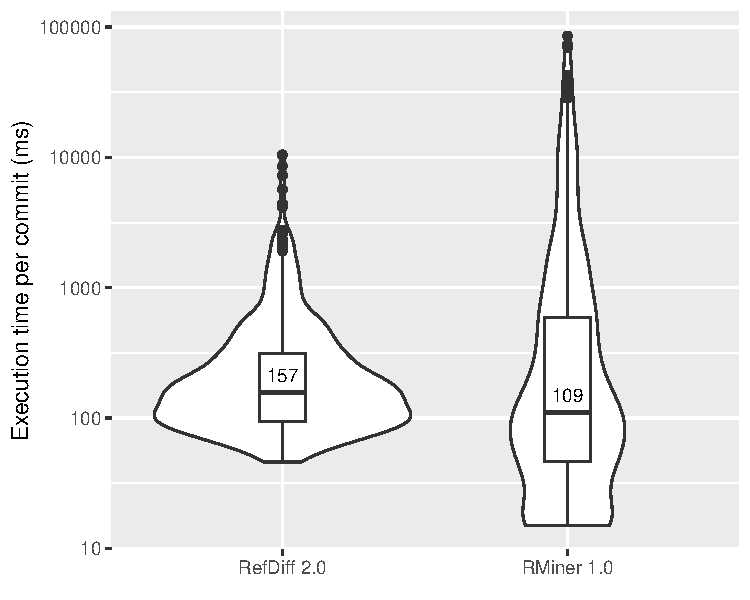
\includegraphics[width=1.0\linewidth]{img-vioplot-exec-time.pdf}
\caption{Violin plot of execution time per commit in log-10 scale}
\label{FigVioplotExecTime}
\end{figure}

\subsection{Threats to Validity}
\label{SecThreatsJava}

There are at least two threats to the validity of the evaluation with Java projects.
The first one is the subjectivity inherent to the manual classification of the reported refactorings as true/false positives, which directly impact the computed precision.
Different validators may have a different interpretation of the code change under analysis, which is demonstrated by the fact that in 34\% of the cases the validators initially disagreed.
We mitigated this threat by having each refactoring assessed by two validators independently.
Second, as discussed in Section~\ref{sec:eval:java:design}, our oracle can not be granted as complete, i.e., there might exist refactorings in the analyzed revisions that are not detected by any of the tools.
Thus, the actual recall might be lower than the computed recall.
Unfortunately, it is not feasible to assure the completeness of an oracle at this scale with manual inspection.
A single commit usually contains hundreds of changed lines of code, making such task extremely time consuming and error prone.
Nevertheless, the computed recall serves the purpose of comparison between tools, and it should also be a fair approximation of actual recall, as our oracle is based on refactorings found by three tools: RMiner~1.0, RefDiff~1.0, and RefDiff~2.0.

%We cannot claim that the precision and recall of our approach would be the same for different projects, with distinct characteristics, and with actual refactorings applied by developers. However, such setup was necessary to compute recall, as discussed in Section~\ref{SecOracleConstruction}. Besides, the results we achieved in the calibration process (precision of 85.7\% and recall of 94.1\%), in which we used actual commits from relevant Java repositories, suggest that RefDiff's precision and recall are acceptable in real scenarios. Nevertheless, we plan to extend this study by assessing the precision of RefDiff in a large corpus of commits from open-source repositories.
%Neverthless, our evaluation includes relevant Java systems of different domains, with up to 374,000 lines of code.
%, and we have no reasons to  believe that precision and recall will be drastically inferior for other systems.
